\scanpage{96}
\figure{\begin{tikzpicture}[x=.78cm,y=.78cm,>=stealth]
\draw (0,-.07) -- (0,1.62) node[left] {$1$};
\fill (0,1.62) circle (.035);
\draw (0,0) -- (1.97,-.01) node[right] {$1$};
\draw (-1.95,2.47) -- (1.87,-1.98);
\draw[->] (-.73,.83) -- (-1.56,1.76);
\draw (-.76,2.04) -- (2.53,-1.48);
\draw (-.74,.83) -- (-1.17,.42) -- (-.46,-.39);
\draw[->,very thick] (-.46,-.43) -- (1.92,1.52);
\draw[->,very thick] (0,0) -- (1.91,-1.99) node[below right] {$a$};
\draw (1.84,-.39) -- (1.77,-1.77);
\fill (0,0) circle (.045) (-.46,-.43) circle (.085) (.51,.46) circle (.085) (-1.17,.42) circle (.075);
\draw (2.53,-1.48) circle (.05);
\node at (-.85,2.13) {$\unsure{o|0}$};
\node[right] at (1.92,1.57) {$\unsure{a|x}$};
\node[right] at (.55,.42) {$s_0$};
\node[below] at (-.58,-.50) {$-s_0$};
\node[left] at (-1.36,.12) {$-s'_0$};
\node at (-1.81,-.34) {$\parallel$};
\node[left] at (-1.23,-.88) {$-(s_0+\tfrac12a)$};
\end{tikzpicture}}
\[
s_0:\ \deleted{\unsure{\zeta|x|X}}\left(\frac1{2-\alpha},\frac1{2-\alpha}\right)=\left(\frac14,\frac14\right)
\]
\[
\begin{aligned}
u&=-(\mathrm{id}+v_0)\\
u^2&=\mathrm{id}+2v_0\\
\left\{\begin{aligned}u^{2n}&=\mathrm{id}+2n v_0\\u^{2n+1}&=-(\mathrm{id}+(2n+1)v_0)\end{aligned}\right.
\end{aligned}
\]
\[
s_{2n}=s_0+2n\underbrace{v_0(s_0)}_{(\frac12,-\frac12)}
=s_0+n\underbrace{(1,-1)}_a=s_0+na
\]
\[
s_{2n+1}=-(s_0+(2n+1)v_0(s_0))=-s_0\unsure{-|+}(n+\tfrac12)a
=(-s_0\unsure{-|+}\tfrac12a)\unsure{-|+}na
\]
\begin{center}\rule{1.7cm}{.35pt}\\[-1.5ex]\rule{1.2cm}{.35pt}\end{center}
III) \uline{$\alpha=+2$} \quad (Pas de centre) \quad $\unsure{\zeta|\rho}=\zeta'=+1$
\[
\begin{aligned}
\deleted{u_V\ \text{d'ordre }p}\qquad u_V&=\mathrm{id}+v_0\qquad v_0=a'\otimes a\ne0,\quad \unsure{u|v}_0^2=0\\
u_V&\ \text{d'ordre }p
\end{aligned}
\]
Je dis que $u_E$ d'ordre $p$, sauf si $p=2$ (déjà traité, où on trouve $2p=4$)
\deleted{$u_E$} Du point de vue de l'enveloppe vectorielle
\[
\begin{aligned}
u_E&=\mathrm{id}+w &w^3&=0\\
u_E^p&=\mathrm{id}+\deleted{\unsure{p}}w^p \quad\deleted{\unsure{pour|si}\ p\unsure{>}} &p\ge3&\quad\text{on gagne}
\end{aligned}
\]
\deleted{$p=2$ on trouve} [pour $p=2$, on trouve $u_E^2=\mathrm{id}+w^2\ne\mathrm{id}$ \unsure{donc|car} $w^2\ne0$]
% archive sheet number: 95
